\section{From Laws to Capability-Specific Selection}
\label{sec:selection}


Given a reference model, a capability, and a budget, which method
and setting preserves that capability best? We write the decision as
\begin{equation}
(m^{*},\boldsymbol\theta_m^{*})=\arg\min_{m,\;\boldsymbol\theta_m\in\mathcal F_m(B)}\;
\widehat L_{m,c}(\mathbf x,\boldsymbol\theta_m),
\label{eq:selection}
\end{equation}
where $\mathcal F_m(B)$ is the set of settings of method $m$ within
budget $B$. 

Two kinds of evidence are kept apart: a retrospective validation of
the laws as selectors and a prospective confirmation of one locked
rule.

\paragraph{Retrospective validation.} On the controlled panel (17
states, storage budgets from 0.2 to 1, every law refit with the
target held out) the law-based choice is within 0.19, 0.17, and 0.42
nats of the oracle for math, code, and QA, picking the oracle's method
in 96\%, 95\%, and 73\% of 289 cells; quantization-only is close
behind (0.21, 0.19, 0.49) because it dominates math and code on this
storage axis (Appendix~\ref{sec:app_selection}).

\paragraph{Prospective confirmation of a locked rule.} We then locked
the complete rule of Table~\ref{tab:final}, froze every candidate's
predicted loss and the four maps for four fresh Pythia states (160M,
410M, and 1.4B at step 32k; 1B at step 64k; 18 configurations each,
weights hashed against every earlier revision), and only then
measured (Fig.~\ref{fig:rule_main}). Over 17 budgets on each state (68 cells per objective from four
models), the locked-rule maps are within 0.00001, 0.004, and 0.14
nats of the oracle for math, code, and QA (2Wiki), below the earlier
source-conditioned maps (0.015, 0.11, 0.21) and quantization-only
under the same candidates, predictor, and feasibility rule (0.007,
0.010, 0.25), meeting the pre-stated criterion; for the largest loss
increase the evaluation is prospective and its criterion was not met
(0.0020 against 0.0019; quantization-only 0.008). The
QA confirmation is an aggregate: the locked rule beats
quantization-only on three states (0.05, 0.24, 0.05 against 0.22,
0.39, 0.28) and trails it on 160M@32k (0.22 against 0.13).  The pruning and quantization candidates are new measurements; the
distillation candidates are two existing same-stage students, purged
from the fit that predicts them, so the round is a selection test, not
a new training experiment. 

\begin{figure}[t]
\centering
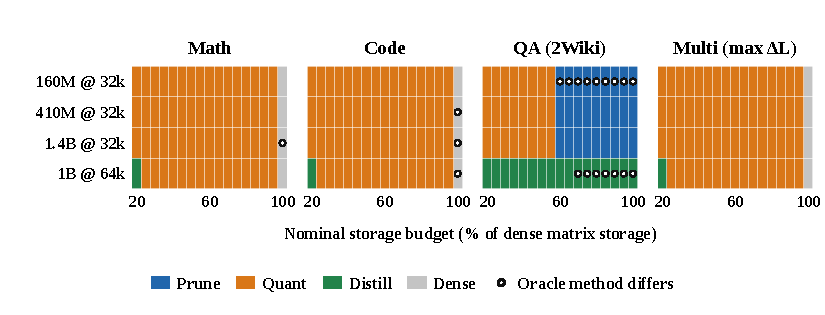
\includegraphics[width=0.8\textwidth]{figs/rule_maps_main.pdf}
\caption{Selection maps under the locked rule on four fresh states (colour = predicted method; marker only where the oracle's method differs). Math and code select quantization almost everywhere; QA (2Wiki) selects pruning at high budgets on the 32k states and distillation on 1B@64k.}
\label{fig:rule_main}
\end{figure}
